\documentclass[11pt,a4paper]{article}
\usepackage{fullpage}
\usepackage[T1]{fontenc} 
\usepackage[utf8]{inputenc}
\usepackage{amsmath}
\usepackage{amssymb}
\usepackage{subcaption}
\usepackage{float}
\usepackage{tabularx}
\usepackage{multirow}
\usepackage{graphicx}
\usepackage{geometry}
\usepackage[table,dvipsnames]{xcolor}
\usepackage[hidelinks]{hyperref}
\usepackage[polish]{babel}
\usepackage{menukeys}

\def\arraystretch{1.5}
\newcolumntype{Y}{>{\centering\arraybackslash}X}
\renewcommand{\thesection}{\arabic{section}.}
\renewcommand{\thesubsection}{\thesection\arabic{subsection}.}
\renewcommand{\thesubsubsection}{\thesubsection\arabic{subsubsection}.}
\setlength{\parindent}{0cm}
\setlength{\parskip}{2mm}

\begin{document}

\title{Metody sztucznej inteligencji 2 \\
\Large{
    Projekt 2. --- Rozpoznawanie kształtów w czasie rzeczywistym \\
    Raport końcowy
}}
\author{Bartłomiej Dach \and Tymon Felski}
\maketitle

Poniższy dokument zawiera końcowy opis projektu, którego celem jest zaimplementowanie rozwiązania pozwalającego na~detekcję i~rozpoznawanie prostych kształtów na~obrazach za~pomocą metod geometrycznych oraz z~użyciem sieci neuronowych i~porównanie skuteczności oraz~wydajności obu wariantów.

\section{Opis problemu badawczego}

Zagadnienie rozpoznawania obiektów na~obrazach z~użyciem metod sztucznej inteligencji stanowi duży obszar zainteresowań naukowych.
Efektywne rozwiązanie tego zagadnienia pomogłoby usprawnić wiele procesów, dotychczas wymagających ludzkiej kontroli i~interwencji.

W~niniejszym projekcie zbiór rozpoznawanych typów obiektów został zawężony do~czterech rodzajów kształtów geometrycznych: trójkąta, kwadratu, koła i~gwiazdy pięcioramiennej (patrz rys, \ref{fig:shapes}).
Kształty mogą znajdować się w~dowolnej orientacji i~mieć dowolny rozmiar.
Dla~uproszczenia zakładamy również, że kolor rozpoznawanych obiektów jest jednakowy i~znany \emph{a~priori}.

\begin{figure}[H]
    \centering
    \begin{subfigure}[t]{0.2\textwidth}
        \centering
        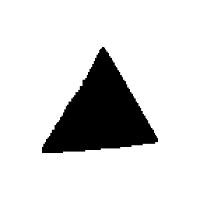
\includegraphics[width=\textwidth]{res/img/triangle.png}
    \end{subfigure}
    \begin{subfigure}[t]{0.2\textwidth}
        \centering
        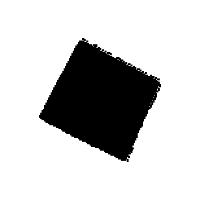
\includegraphics[width=\textwidth]{res/img/square.png}
    \end{subfigure}
    \\
    \begin{subfigure}[t]{0.2\textwidth}
        \centering
        
\includegraphics[width=\textwidth]{res/img/star.png}
    \end{subfigure}
    \begin{subfigure}[t]{0.2\textwidth}
        \centering
        
\includegraphics[width=\textwidth]{res/img/circle.png}
    \end{subfigure}
    \caption{Przykładowe kształty ze~zbioru treningowego używanego do~treningu i~oceny jakości klasyfikatorów}
    \label{fig:shapes}
\end{figure}

\subsection{Cel badań}

Kształty geometryczne wykazują pewien stopień regularności, co~powoduje, że do~ich rozpoznawania można próbować zastosować algorytmy dokładne.
Przykładem są zaimplementowane w~bibliotece OpenCV \cite{opencv}:
\begin{itemize}
    \item algorytm Suzukiego \cite{suzuki1985} do~wyznaczania konturów na~podstawie obrazów rastrowych,
    \item algorytm Douglasa-Peuckera \cite{douglas1973} do~upraszczania konturów i~redukcji liczby punktów.
\end{itemize}
Dzięki tym dwóm algorytmom można na~podstawie binarnego obrazu wejściowego wyznaczyć kontur kształtu --- łamaną zamkniętą przybliżającą kształt wyznaczony przez piksele kształtu na~tle.

Oprócz metod dokładnych, do~zagadnienia rozpoznawania można również użyć sieci neuronowych, które zamiast wiedzy dokładnej używają przygotowanych zbiorów treningowych oraz metod optymalizacji, aby~dokonać klasyfikacji.
Celem badań jest porównanie wydajności i~skuteczności wybranych metod.

\subsection{Wykorzystane techniki}

Do~zaimplementowania klasyfikatorów użyty został język skryptowy \textbf{Python} w~wersji 3.5.2.
Ponadto wykorzystane zostały dodatkowe biblioteki, wymienione w~tabeli~\ref{tbl:libraries}.
Podejście geometryczne opiera~się na~funkcjach udostępnianych przez \textbf{OpenCV}, podczas gdy sieci neuronowe stworzone zostały za~pośrednictwem API dostarczanego przez bibliotekę \textbf{Keras}.

\begin{table}[H]
    \begin{tabularx}{\textwidth}{|c|l|X|l|c|}
        \hline
        \textbf{Nr} & \textbf{Komponent, wersja} & \textbf{Opis} & \textbf{Licencja} & \\
        \hline
        \hline
        1 &
        h5py, 2.7.1 &
        Interfejs dla binarnego formatu danych HDF5, wymagany przez Keras &
        BSD License &
        \cite{h5py} \\
        \hline
        2 &
        Keras, 2.1.4 &
        Biblioteka udostępniająca API do~sieci neuronowych &
        MIT License &
        \cite{keras} \\
        \hline
        3 & 
        Matplotlib, 2.1.0 & 
        Umożliwia tworzenie wykresów &
        Matplotlib License &
        \cite{matplotlib} \\
        \hline
        4 & 
        NumPy, 1.13.3 &
        Używana do~efektywnych obliczeń na~wektorach $n$-wymiarowych &
        BSD License &
        \cite{numpy} \\
        \hline
        5 & 
        OpenCV, 3.3.0 &
        Biblioteka do~obróbki obrazów &
        New BSD License &
        \cite{opencv} \\
        \hline
        6 &
        pandas, 0.21.0 &
        Wspomaga ładowanie danych z~plików CSV oraz~ich analizę &
        BSD License &
        \cite{pandas} \\
        \hline
        7 &
        TensorFlow, 1.8.0 &
        Framework do~uczenia maszynowego używany przez Keras &
        Apache 2.0 &
        \cite{tensorflow} \\
        \hline
    \end{tabularx}
    \caption{Wykorzystane biblioteki wraz z~określeniem licencji}
    \label{tbl:libraries}
\end{table}

\subsubsection{Wycięcie kształtów z~tła}

Ponieważ projekt zakłada, że kolor kształtów jest zadany z~góry, do~ekstrakcji kształtów z~tła wystarczy zastosować operację progowania obrazu.
Pozwala ona na~zamianę obrazu w~kolorze na~obraz binarny.
Progowanie wykonywane jest w~przestrzeni kolorów HSV, która dobrze odwzorowuje podobieństwo odcieni barw; wystarczy zdefiniować przedział dla~parametru H, który określa sąsiedztwo tonalne żądanego koloru.

\subsubsection{Klasyfikator geometryczny}

Główną ideą działania klasyfikatora geometrycznego jest dopasowanie łamanej zamkniętej do~rozpoznanego kształtu i~analiza kształtu tej łamanej.

Do~odróżniania kształtów wykorzystywana jest przede wszystkim liczba wierzchołków w~wyznaczonym konturze.
Pozwala ona na~proste odróżnienie trójkątów, czworokątów i~dziesięciokątów od~pozostałych kształtów.
Ponadto, dla~każdego kształtu innego niż trójkąt, stosowane~są odpowiednie heurystyki:

\begin{itemize}
    \item W~przypadku kwadratów, sprawdzana jest proporcja wysokości do~szerokości kształtu (powinna być bliska jedności).
    Ponadto bok kwadratu wyznaczany jest na~podstawie pola i~obwodu figury; jeśli dwie wyznaczone wartości nie są bliskie sobie, kształt jest odrzucany.
    \item Rozpoznawanie gwiazd korzysta z~faktu, że wierzchołki parzyste i~nieparzyste gwiazdy znajdują~się w~innych odległościach od~środka figury.
    Zatem, jeśli odchylenie standardowe odległości od~środka wierzchołków parzystych i nieparzystych jest zbyt duże, figura jest odrzucana.
    \item Dla~kół, podobnie jak dla~kwadratów, promień koła wyznaczany jest dwukrotnie na~podstawie pola i~obwodu figury.
    W~przypadku zbyt dużej różnicy kształt nie jest klasyfikowany.
\end{itemize}

\subsubsection{Klasyfikatory oparte na~sieciach neuronowych}

Klasyfikatory oparte na~sieciach były trenowane na~podstawie zbioru treningowego \cite{shapes}.
Zostały opracowane dwa warianty sieci, operujące na~obrazie wejściowym rozmiarów $64 \times 64$:

\begin{itemize}
    \item W~pierwszym wariancie wejściowy binarny obraz dwuwymiarowy spłaszczany jest do~jednowymiarowego wektora, który przekazywany jest na~wejście sieci.
    Użyta sieć korzysta z~trzech warstw ukrytych z~funkcją aktywacji ReLU (ang. \emph{Rectified Linear Unit}).
    Ponadto, po~każdej warstwie ukrytej dodana jest warstwa \emph{dropout}, zapobiegająca zjawisku \emph{overfitting} \cite{srivastava2014}.

    Warstwa wyjściowa jako funkcji aktywacji używa funkcji \emph{softmax}.
    \item Drugi wariant korzysta z~pojedynczej warstwy konwolucyjnej z~rozmiarem okna $8 \times 8$ oraz warstwy \emph{dropout}.
    Wynik warstwy konwolucyjnej jest spłaszczany i~dostarczany do~warstwy wyjściowej z~funkcją \emph{softmax}.
\end{itemize}

\section{Instrukcja użytkowania}

W~skład projektu wchodzą trzy główne skrypty Pythona, odpowiadające kolejno za~trenowanie klasyfikatorów opartych na~sieciach neuronowych i~testowanie działania wszystkich trzech klasyfikatorów na~obrazach statycznych oraz strumieniach wideo z~kamery komputera. 

\subsection{Trenowanie sieci neuronowej}

Do~wykonania treningu sieci neuronowej należy wykorzystać skrypt \verb+train.py+.
Dokonuje on wyznaczenia modelu dla~sieci w~obu wariantach (spłaszczonym i~konwolucyjnym).
Skrypt należy wywołać poleceniem
\begin{verbatim}
$ python train.py -d train-image-directory
\end{verbatim}
gdzie \verb+train-image-directory+ oznacza katalog zawierający zbiór treningowy udostępniony w~\cite{shapes}.
Obrazy w~zbiorze treningowym muszą zawierać czarne kształty na~białym tle.

Wykonanie skryptu rozpocznie proces uczenia sieci, który może potrwać do~kilkunastu minut.
W~wyniku działania skryptu w~bieżącym katalogu zostanie stworzony podkatalog \verb+model+, zawierający dwa pliki:

\begin{itemize}
    \item Plik \verb+shapes_model_1d_vec.h5+ zawiera model dla~sieci neuronowej operującej na~spłaszczonym obrazie wytrenowany przy użyciu 50 epok.
    \item Plik \verb+shapes_model_2d_img.h5+ zawiera model dla~konwolucyjnej sieci neuronowej wytrenowany przy użyciu 25 epok.
\end{itemize}

\subsection{Testy na~obrazach wczytywanych z~pliku}

Klasyfikacji dla~folderu zawierającego obrazy można wykonać za~pomocą skryptu \verb+image_test.py+.
Skrypt ten wczyta wszystkie obrazy (z białymi kształtami na~czarnym tle) znajdujące~się w~danym folderze i~dokona ich zbiorczej identyfikacji.
Do~uruchomienia go należy użyć polecenia
\begin{verbatim}
$ python image_test.py -d test-image-directory
                       -c {geometric,vector-network,convolutional-network}
\end{verbatim}

\begin{itemize}
    \item W~parametrze \verb+-d+ podajemy ścieżkę do~folderu, w~którym znajdują~się obrazy testowe.
    \item Parametr \verb+-c+ służy wyborowi klasyfikatora, który powinien być użyty dla~danych testowych.
    Możliwe opcje to:
    \begin{itemize}
        \item \verb+geometric+ --- używa klasyfikatora geometrycznego,
        \item \verb+vector-network+ --- używa klasyfikatora opartego o~płaską sieć neuronową,
        \item \verb+convolutional-network+ --- używa klasyfikatora opartego o~sieć konwolucyjną.
    \end{itemize}
\end{itemize}

Na~wyjściu program wypisze liczbę rozpoznanych kształtów każdego rodzaju na~wszystkich obrazach znajdujących~się w~wyspecyfikowanym katalogu.

\subsection{Rozpoznawanie kształtów w~czasie rzeczywistym}

Ostatni skrypt, \verb+capture.py+, służy demonstracji działania klasyfikatorów na~strumieniu wideo.
Obraz pobierany jest z~kamerki komputera, jeśli taką posiada.
Skrypt uruchamiamy bez parametrów poleceniem:
\begin{verbatim}
$ python capture.py
\end{verbatim}
Skrypt ma~charakter interaktywnego okna --- za~pomocą klawiszy klawiatury można przełączać~się między klasyfikatorami lub dokonać próby czasowej.
Dokładny opis wszystkich opcji znajduje~się poniżej.

\begin{itemize}
    \item Klawisze numeryczne służą przełączaniu~się między klasyfikatorami, których wyniki wyświetlane~są na~podglądzie.
    \begin{itemize}
        \item Klawisz \keys{1} powoduje przełączenie podglądu na~klasyfikator geometryczny.
        \item Klawisz \keys{2} powoduje przełączenie podglądu na~wektorowy klasyfikator z~siecią neuronową.
        \item Klawisz \keys{3} powoduje przełączenie podglądu na~klasyfikator z~konwolucyjną siecią neuronową.
    \end{itemize}
    \item Za~pomocą skryptu można wykonać próbę czasową wszystkich klasyfikatorów dla~ustalonego rodzaju kształtu.
    Dla~każdego klasyfikatora liczony jest czas poprawnej klasyfikacji.
    Czas zatrzymywany jest, jeśli klasyfikator przez dłużej niż~8~klatek podejmował próbę rozpoznania kształtu i rozpoznawał inny kształt niż był ustawiony obecnie oczekiwany lub gdy stwierdził, że wykryty obszar nie zawiera żadnego ze znanych mu kształtów.
    \begin{itemize}
        \item Klawisze \keys{Z}, \keys{X}, \keys{C}, \keys{V} pozwalają zmienić rodzaj kształtu.
        \begin{itemize}
            \item Wciśnięcie klawisza \keys{Z} spowoduje, że oczekiwanym kształtem będzie kwadrat.
            \item Wciśnięcie klawisza \keys{X} spowoduje, że oczekiwanym kształtem będzie gwiazda.
            \item Wciśnięcie klawisza \keys{C} spowoduje, że oczekiwanym kształtem będzie koło.
            \item Wciśnięcie klawisza \keys{V} spowoduje, że oczekiwanym kształtem będzie trójkąt.
        \end{itemize}
        \item Klawisz \keys{A} powoduje rozpoczęcie próby czasowej.
        \item Klawisz \keys{S} powoduje zatrzymanie rozpoczętej próby czasowej.
        \item Klawisz \keys{R} powoduje zrestartowanie próby czasowej.
    \end{itemize}
    Podczas trwania próby można zarówno zmieniać docelowy typ rozpoznawanego kształtu, jak i~przełączać podgląd wyników klasyfikatora między dostępnymi opcjami.
    \item Klawisz \keys{H} powoduje wyświetlenie pomocy na~ekranie.
    \item Klawisz \keys{D} powoduje włączenie trybu \emph{debug}.
    W~tym trybie w~osobnym oknie na~ekranie wyświetlane~są rozpoznawane po~progowaniu kontury, a na~konsoli wyświetlane są: średni, minimalny i maksymalny czas działania poszczególnych klasyfikatorów.
    \item Klawisz \keys{Q} powoduje zakończenie działania skryptu.
\end{itemize}

\section{Wyniki eksperymentalne}

W~celu oceny zaimplementowanych klasyfikatorów wykonane zostało kilka eksperymentów, których celem było zbadanie ich efektywności i~wydajności.
Niniejszy rozdział zawiera opis wykonanych testów oraz~przedstawia uzyskane wyniki.

\subsection{Kryteria oceny klasyfikatorów}

Ocenie zdecydowano się poddać kilka kryteriów. Wyniki klasyfikacji postanowiono zbadać poprzez wyznaczenie dokładności \emph{(ang. accuracy)}, która jest jedną z miar oceny jakości klasyfikacji. Wydajność klasyfikatorów zweryfikowano mierząc czas wywołań klasyfikacji dla każdego z~nich. Ponadto klasyfikatory poddano próbie o~charakterze empirycznym, polegającej na~teście w~czasie rzeczywistym. 

\subsubsection{Dokładność}

Dokładność jest najbardziej intuicyjnym pojęciem pozwalającym na zmierzenie szeroko rozumianej skuteczności klasyfikatora. Dokładność jest bowiem stosunkiem liczby poprawnych klasyfikacji do~liczby rozpoznawanych kształtów.

Dla każdego obrazu ze zbioru \cite{shapes} uruchomiono klasyfikację kształtu przy pomocy klasyfikatora geometrycznego i każdej z sieci neuronowych. Następnie zgodnie z definicją dokładności zliczono poprawne wyniki i wyznaczono szukany współczynnik.

W przypadku rozpatrywanych sieci neuronowych dokładność jest dodatkowo jedną z miar wypisywanych na ekran w trybie \emph{verbose} podczas treningu. Podczas trenowania zbiór danych wejściowych dzielony jest na dwa zbiory --- co piąty element odkładany jest na bok do zbioru testowego. Zbiór treningowy zawiera wobec tego 80\% obrazów, a po każdej epoce następuje walidacja obecnego stanu sieci przy pomocy pozostałych 20\% obrazów. Na samym końcu treningu wykonywana jest ewaluacja wytrenowanego modelu, w celu ustalenia ostatecznej dokładności klasyfikacji na zbiorze testowym.

\subsubsection{Wydajność}

Stworzony na potrzeby projektu skrypt \verb+capture.py+ pozwala na włączenie trybu \emph{debug}, dzięki któremu wyniki wydajnościowe każdego klasyfikatora są wypisywane na ekran. Podawane są~wartości takie jak:
\begin{itemize}
    \item minimalny czas klasyfikacji od początku działania skryptu,
    \item maksymalny czas klasyfikacji od początku działania skryptu,
    \item średni czas klasyfikacji od początku działania skryptu.
\end{itemize}
Zdecydowano się nie liczyć mediany, ponieważ wymagałoby to zapamiętania wszystkich czasów klasyfikacji, co~wpłynęłoby negatywnie na~zużycie pamięci.

\subsubsection{Próba czasowa}

W~tym teście zbadano zachowanie wszystkich trzech klasyfikatorów jednocześnie w~tym samym scenariuszu, obejmującym rozpoznawanie kształtów w~czasie rzeczywistym na~strumieniu wideo. Wykorzystano w~tym celu opisywany wcześniej skrypt \verb+capture.py+, przy pomocy którego ustawiono na~rozpoznawanie konkretnego kształtu i~uruchomiono próbę czasową. Zadaniem jest poprawna klasyfikacja pokazywanego kształtu przez jak najdłuższy okres czasu, przy czym dopuszcza~się pomyłkę przez nie~dłużej niż 8~klatek z~rzędu. Zwrócenie błędnego wyniku przez dłużej niż~ustalony limit powoduje zakończenie pomiaru czasu dla~danego klasyfikatora.

\subsection{Uzyskane wyniki}

W poniższym podrozdziale opisano wyniki uzyskane przy pomocy opisanych powyżej testów.

\subsubsection{Dokładność}

W zbiorze \cite{shapes} znajduje się 14970 obrazów --- 3720 kół, 3765 kwadratów, 3765 gwiazd i 3720 trójkątów. Dla każdego z klasyfikatorów wyznaczono dokładność uruchamiając proces klasyfikacji na każdym z obrazów przy pomocy skryptu \verb+image_test.py+ i zliczając stosunek poprawnych dopasowań do liczby wszystkich prób. Wyniki wyglądają następująco:
\begin{itemize}
    \item Klasyfikator geometryczny zakwalifikował poprawnie 14911 kształtów, co daje dokładność na poziomie 0.9961 w przybliżeniu.
    W~tym przypadku najgorzej wypadły trójkąty --- były tam aż~153 pomyłki.
    \item Klasyfikator korzystający z sieci neuronowej klasyfikującej wektory zidentyfikował poprawnie 14813 kształtów, co daje dokładność na~poziomie 0.9895. Najwięcej błędów zostało popełnionych w~przypadku klasyfikacji gwiazd (46).
    \item Klasyfikator korzystający z konwolucyjnej sieci neuronowej rozpoznał poprawnie 14915 kształtów, co daje dokładność na poziomie 0.9963 w przybliżeniu. Podobnie jak w~przypadku klasyfikatora geometrycznego, najgorzej wypadła klasyfikacja trójkątów (53 pomyłki).
\end{itemize}

Warto zauważyć, że poza siedmioma przypadkami błędnej identyfikacji trójkątów jako kwadraty i~gwiazdy przez sieć konwolucyjną, nie wystąpiły żadne błędy pierwszego typu (ang. \emph{false positive errors}). Wszystkie popełnione błędy dotyczyły nierozpoznania znanego kształtu.

Jak już wspomniano wcześniej, dokładność była także wypisywana na ekran w trakcie treningu sieci neuronowych. Wartość wyznaczona podczas ewaluacji wytrenowanego modelu w~przypadku sieci klasyfikującej wektory to 0.9980, natomiast dla sieci konwolucyjnej zwrócona wartość była 1.0 (wyniosła tyle już po siedemnastej z 25 epok).

\subsubsection{Wydajność}

Wydajność każdej z metod klasyfikacji zmierzono na dwa sposoby. Pierwszym źródłem wyników był wykorzystany do badania dokładności skrypt \verb+image_test.py+, w którym zmierzono upływ czasu klasyfikacji wszystkich 14970 obrazów łącznie z ich obróbką przez ekstraktor (komponent programu znajdujący figury na~obrazie). Otrzymane wyniki są następujące:
\begin{itemize}
    \item Klasyfikator geometryczny skończył klasyfikację obrazów w 28.66s, co daje w przybliżeniu średnio 0.0019s na obróbkę i klasyfikację każdego kształtu.
    \item Klasyfikator korzystający z sieci neuronowej klasyfikującej wektory skończył klasyfikację obrazów w 43.67s, co daje w przybliżeniu średnio 0.0029s na obróbkę i klasyfikację każdego kształtu.
    \item Klasyfikator korzystający z konwolucyjnej sieci neuronowej skończył klasyfikację obrazów w 48.53s, co daje w przybliżeniu średnio 0.0032s na obróbkę i klasyfikację każdego kształtu.
\end{itemize}

Drugim źródłem wyników był działający w trybie \emph{debug} skrypt \verb+capture.py+. Dla każdego z klasyfikatorów otrzymano następujące wyniki klasyfikacji pojedynczego kształtu (bez obróbki wstępnej):
\begin{itemize}
    \item Klasyfikator geometryczny:
    \begin{itemize}
        \item najkrótszy czas klasyfikacji wyniósł 0.000018s,
        \item najdłuższy czas klasyfikacji wyniósł 0.001961s,
        \item średni czas klasyfikacji wyniósł 0.000086s.
    \end{itemize}
    \item Klasyfikator korzystający z sieci neuronowej klasyfikującej wektory:
    \begin{itemize}
        \item najkrótszy czas klasyfikacji wyniósł 0.000981s,
        \item najdłuższy czas klasyfikacji wyniósł 0.022804s,
        \item średni czas klasyfikacji wyniósł 0.001918s.
    \end{itemize}
    \item Klasyfikator korzystający z konwolucyjnej sieci neuronowej:
    \begin{itemize}
        \item najkrótszy czas klasyfikacji wyniósł 0.001086s,
        \item najdłuższy czas klasyfikacji wyniósł 0.035751s,
        \item średni czas klasyfikacji wyniósł 0.002212s.
    \end{itemize}
\end{itemize}

\subsubsection{Próba czasowa}

Testom poddano każdy z kształtów osobno przy dodatkowym zastosowaniu różnych utrudnień, którymi są:
\begin{itemize}
    \item translacja (przesuwanie) kształtu wzdłuż~płaszczyzny kamery,
    \item obrót kształtu,
    \item przechylenie kształtu względem~płaszczyzny kamery,
    \item przybliżanie i~oddalanie kształtu.
\end{itemize}

Wyniki wykonanych prób czasowych znajdują się w tabeli~\ref{tab:time-trials}. Kolumny oznaczone jako \emph{geometric}, \emph{network (vec)} oraz \emph{network (conv)} odpowiadają odpowiednio klasyfikatorom: geometrycznemu, opartemu na sieci neuronowej klasyfikującej wektory oraz sieci konwolucyjnej.

\begin{table}[H]
    \begin{tabularx}{\textwidth}{|c|c|Yr|Yr|Yr|}
        \hline
        \textbf{Test} & \textbf{Kształt} & \multicolumn{2}{c|}{\textbf{geometric}} & \multicolumn{2}{c|}{\textbf{network (vec)}} & \multicolumn{2}{c|}{\textbf{network (conv)}} \\
        \hline
        \hline
        \multirow{4}{*}{\rotatebox[origin=c]{90}{\textbf{Translacja}}}
        & kwadrat & 00:14.368 & \footnotesize{(0.960)} & 00:14.968 & \footnotesize{(1.000)} & 00:14.968 & \footnotesize{(1.000)} \\
        \cline{2-8}
        & koło & 00:16.493 & \footnotesize{(1.000)} & 00:16.493 & \footnotesize{(1.000)} & 00:16.493 & \footnotesize{(1.000)} \\
        \cline{2-8}
        & trójkąt & 00:13.210 & \footnotesize{(1.000)} & 00:13.210 & \footnotesize{(1.000)} & 00:13.210 & \footnotesize{(1.000)} \\
        \cline{2-8}
        & gwiazda & 00:14.480 & \footnotesize{(1.000)} & 00:14.480 & \footnotesize{(1.000)} & 00:14.480 & \footnotesize{(1.000)} \\
        \hline
        \hline
        \multirow{4}{*}{\rotatebox[origin=c]{90}{\textbf{Obrót}}}
        & kwadrat & 00:17.291 & \footnotesize{(1.000)} & 00:17.291 & \footnotesize{(1.000)} & 00:17.291 & \footnotesize{(1.000)} \\
        \cline{2-8}
        & koło & 00:17.936 & \footnotesize{(1.000)} & 00:17.936 & \footnotesize{(1.000)} & 00:17.936 & \footnotesize{(1.000)} \\
        \cline{2-8}
        & trójkąt & 00:18.347 & \footnotesize{(1.000)} & 00:18.347 & \footnotesize{(1.000)} & 00:18.347 & \footnotesize{(1.000)} \\
        \cline{2-8}
        & gwiazda & 00:10.154 & \footnotesize{(0.652)} & 00:10.231 & \footnotesize{(0.657)} & 00:15.575 & \footnotesize{(1.000)} \\
        \hline
        \hline
        \multirow{4}{*}{\rotatebox[origin=c]{90}{\textbf{Przechylenie}}}
        & kwadrat & 00:03.113 & \footnotesize{(0.495)} & 00:06.254 & \footnotesize{(0.995)} & 00:06.285 & \footnotesize{(1.000)} \\
        \cline{2-8}
        & koło & 00:05.658 & \footnotesize{(0.983)} & 00:05.568 & \footnotesize{(0.968)} & 00:05.753 & \footnotesize{(1.000)} \\
        \cline{2-8}
        & trójkąt & 00:14.188 & \footnotesize{(1.000)} & 00:14.188 & \footnotesize{(1.000)} & 00:04.518 & \footnotesize{(0.318)} \\
        \cline{2-8}
        & gwiazda & 00:08.886 & \footnotesize{(0.651)} & 00:03.590 & \footnotesize{(0.263)} & 00:13.652 & \footnotesize{(1.000)} \\
        \hline
        \hline
        \multirow{4}{*}{\rotatebox[origin=c]{90}{\textbf{Przybliżenie}}}
        & kwadrat & 00:17.115 & \footnotesize{(1.000)} & 00:17.115 & \footnotesize{(1.000)} & 00:17.115 & \footnotesize{(1.000)} \\
        \cline{2-8}
        & koło & 00:08.984 & \footnotesize{(0.982)} & 00:09.150 & \footnotesize{(1.000)} & 00:08.921 & \footnotesize{(0.975)} \\
        \cline{2-8}
        & trójkąt & 00:04.483 & \footnotesize{(0.289)} & 00:15.498 & \footnotesize{(1.000)} & 00:15.498 & \footnotesize{(1.000)} \\
        \cline{2-8}
        & gwiazda & 00:04.558 & \footnotesize{(0.319)} & 00:04.590 & \footnotesize{(0.321)} & 00:14.308 & \footnotesize{(1.000)} \\
        \hline
    \end{tabularx}
    \caption{Wyniki przeprowadzonych prób czasowych.
    W~nawiasach stosunek do~najlepszego wyniku w~obrębie danego wiersza.}
    \label{tab:time-trials}
\end{table}

Dla~każdego z~uzyskanych czasów obliczony został jego stosunek do~najlepszego wyniku uzyskanego przez~klasyfikatory w~danej próbie.
W~tabeli \ref{tab:average-ratio} widoczny jest średni stosunek do~najlepszego wyniku z~wszystkich prób dla~poszczególnych klasyfikatorów.

\begin{table}[H]
    \centering
    \begin{tabularx}{0.6\textwidth}{|l|Y|}
        \hline
        \textbf{Klasyfikator} & \textbf{Średni stosunek} \\
        \hline
        geometric & 0.833 \\
        \hline
        network (vec) & 0.888 \\
        \hline
        network (conv) & 0.956 \\
        \hline
    \end{tabularx}
    \caption{Uśrednione wyniki względne z~prób przedstawionych w~tabeli \ref{tab:time-trials}}
    \label{tab:average-ratio}
\end{table}

W~teście empirycznym najlepiej zaprezentowała~się sieć konwolucyjna, ze~względu na~największą stabilność działania.

\section{Podsumowanie}

Przeprowadzone eksperymenty pokazują, że~wszystkie zastosowane podejścia dość dobrze radzą sobie z~problemem rozpoznawania prostych kształtów.
Zauważalne są jednak między nimi różnice w~dziedzinie wydajności i~efektywności.

Klasyfikator oparty na~konturach wykazuje w~eksperymentach najkrótszy czas działania, lecz często działa dość niestabilnie, co~wykazała próba czasowa.
Z~kolei sieci neuronowe mimo konieczności treningu na~wcześniej przygotowanym zbiorze oraz dłuższego czasu klasyfikacji, nadal mogą być używane do~rozpoznawania w~czasie rzeczywistym, i~działają mniej chaotycznie, niż podejście typowo geometryczne.

\subsection{Możliwości dalszych badań}

Istnieje kilka potencjalnych zagadnień, stanowiących naturalną kontynuację opracowanego projektu:

\begin{itemize}
    \item Naturalnym rozszerzeniem istniejącego rozwiązania byłoby dodanie większej liczby rodzajów rozpoznawanych kształtów.
    Koszt takiego rozszerzenia różniłby~się znacząco pomiędzy klasyfikatorami --- podczas gdy rozszerzenie klasyfikatora geometrycznego byłoby stosunkowo bezproblemowe, dla~pozostałych dwóch należałoby przygotować zbiór treningowy oraz~ponownie wytrenować model sieci.
    \item Interesującym aspektem analizy stworzonych rozwiązań byłaby również ocena ich podatności na~błędy pierwszego rodzaju (ang. \emph{false positive}).
    Znane są rozwiązania używające np.~sieci adwersaryjnych (ang. \emph{adversarial network}) w~celu wygenerowania obrazów powodujących błędne działanie klasyfikatorów opartych na~sieciach neuronowych.
    \item Pewną wadą modeli dopasowanych w~ramach projektów jest nieuwzględnienie w~zbiorze treningowych obiektów niepasujących do~żadnej z~kategorii kształtów.
    Wobec tego pomysłem wartym rozważenia byłoby dodanie dodatkowej zbiorczej klasy na~wszystkie pozostałe kształty niepasujące do~ustalonych archetypów.
\end{itemize}

\begin{thebibliography}{99}

    \bibitem{bishop1995}
        C.M. Bishop:
        \emph{Neural Networks for~Pattern Recognition}.
        Oxford University Press:
        Nowy Jork,
        1995.

    \bibitem{keras}
        F. Chollet, Keras Team:
        Keras -- Deep Learning for humans. \\
        Oficjalna strona: \url{https://keras.io}
        [Dostęp 17~marca 2018]

    \bibitem{h5py}
        A. Collette,
        HDF5 for Python. \\
        Oficjalna strona: \url{https://www.h5py.org/}
        [Dostęp 27~maja 2018]
        
    \bibitem{douglas1973}
        D.H. Douglas,
        T.K. Peucker,
        ,,Algorithms for the Reduction of~the~Number of~Points Required to~Represent a~Digitized Line or its Caricature'',
        \emph{Cartographica: The International Journal for Geographic Information and~Geovisualization},
        tom 10,
        s. 112--122,
        1973.

    \bibitem{opencv}
        Intel Corporation, Willow Garage, Itseez:
        OpenCV -- Open Source Computer Vision. \\
        Oficjalna strona: \url{https://opencv.org}.
        [Dostęp 17~marca 2018]

    \bibitem{matplotlib}
        Matplotlib Development Team:
        Matplotlib. \\
        Oficjalna strona: \url{https://matplotlib.org}.
        [Dostęp 17~marca 2018]

    \bibitem{pandas}
        W. McKinney:
        pandas -- Python Data Analysis Library. \\
        Oficjalna strona: \url{https://pandas.pydata.org}.
        [Dostęp 17~marca 2018]

    \bibitem{shapes}
        S. Meschke:
        Four Shapes dataset. \\
        Dostępny: \url{https://www.kaggle.com/smeschke/four-shapes}.
        [Dostęp 17~marca 2018]

    \bibitem{murty2015}
        M.N. Murty,
        V.S. Devi:
        \emph{Introduction to~Pattern Recognition and~Machine Learning}.
        World Scientific Publishing:
        Singapur,
        2015.

    \bibitem{numpy}
        T. Oliphant:
        NumPy. \\
        Oficjalna strona: \url{http://www.numpy.org}.
        [Dostęp 17~marca 2018]
        
    \bibitem{srivastava2014}
        N. Srivastava,
        G. Hinton,
        A. Krizhevsky,
        I. Sutskever,
        R. Salakhutdinov,
        ,,Dropout: A Simple Way to Prevent Neural Networks from Overfitting'',
        \emph{Journal of Machine Learning Research},
        tom 15,
        s.~1929--1958,
        2014.

    \bibitem{suzuki1985}
        S. Suzuki,
        K. Abe,
        ,,Topological structural analysis of~digitized binary images''
        \emph{Computer Vision, Graphics and~Image Processing},
        tom 30,
        s.~32--66,
        1985.

    \bibitem{tensorflow}
        TensorFlow Team:
        TensorFlow -- An open source machine learning framework for everyone. \\
        Oficjalna strona: \url{https://www.tensorflow.org/}
        [Dostęp 27~maja 2018]

\end{thebibliography}

\end{document}